\begin{name}
	{\tenchude}
	{TOÁN 12}
	{LỚP TOÁN THẦY PHÁT}
	{Thời gian: 90 phút - Không kể thời gian phát đề}
\end{name}
\Opensolutionfile{ansbook}[ans/ansbookDe3]
\TN
\Opensolutionfile{ans}[ans/ansDe3-TN1]
\begin{ex}%[Dự án 2025 - đề cấu trúc mới, Nguyễn Kiều Nhã Tú]%[2D4N1-1]
Mệnh đề nào dưới đây \textbf{sai}?
\choice
{$\displaystyle\int f'(x)\mathrm{\,d}x=f(x)+C$ với mọi hàm số $f(x)$ có đạo hàm trên $\mathbb{R}$}
{$\displaystyle\int[f(x)+g(x)]\mathrm{\,d}x=\displaystyle\int f(x) \mathrm{\,d}x+\displaystyle\int g(x)\mathrm{\,d}x$ với mọi hàm số $f(x)$, $g(x)$ có đạo hàm trên $\mathbb{R}$}
{\True $\displaystyle\int kf(x)\mathrm{\,d}x=k\displaystyle\int f(x) \mathrm{\,d}x$ với mọi hằng số $k$ và với mọi hàm số $f(x)$ có đạo hàm trên $\mathbb{R}$}
{$\displaystyle\int[f(x)-g(x)]\mathrm{\,d}x=\displaystyle\int f(x) \mathrm{\,d}x-\displaystyle\int g(x)\mathrm{\,d}x$ với mọi hàm số $f(x)$, $g(x)$ có đạo hàm trên $\mathbb{R}$}
\loigiai{
Theo tính chất của nguyên hàm, $\displaystyle\int kf(x)\mathrm{\,d}x=k \displaystyle\int f(x)\mathrm{\,d}x$ sai khi $k=0$.
}
\end{ex}

\begin{ex}%[2D4N1-2]
Họ nguyên hàm của hàm số $f(x)=x^3$ là
\choice
{$4x^4+C$}
{$3x^2+C$}
{$x^4+C$}
{\True $\dfrac{1}{4}x^4+C$}
\loigiai{
Ta có
$\displaystyle\int x^3\mathrm{\,d}x=\dfrac{1}{4}x^4+C$.
}
\end{ex}

\begin{ex}%[2D4N2-1]
Cho $\displaystyle\int\limits_0^1f(x)\mathrm{\,d}x=2$ và $\displaystyle\int\limits_0^1g(x)\mathrm{\,d}x=5$, khi $\displaystyle\int\limits_0^1\left[f(x)-2g(x)\right]\mathrm{\,d}x$ bằng
\choice
{\True $-8$}
{$1$}
{$-3$}
{$12$}
\loigiai{
Ta có $\displaystyle\int\limits_0^1\left[f(x)-2g(x)\right]\mathrm{\,d}x=\displaystyle\int\limits_0^1f(x)\mathrm{\,d}x-2\displaystyle\int\limits_0^1g(x)\mathrm{\,d}x=2-2\cdot 5=-8$.}
\end{ex}

\begin{ex}%[2H5N1-1]
Trong không gian với hệ tọa độ $O x y z$, phương trình nào sau đây là phương trình của mặt phẳng $O z x$ ?
\choice
{$x=0$}
{$y-1=0$}
{\True $y=0$}
{$z=0$}
\loigiai{
Ta có mặt phẳng $(Oxz)$ đi qua điểm $O(0 ; 0 ; 0)$ và vuông góc với trục $O y$ nên có VTPT $\vec{n}=(0 ; 1 ; 0)$.\\
Do đó phương trình của mặt phẳng $(Oxz)$ là $y=0$.
}
\end{ex}

\begin{ex}%[Mức độ 1]%[BG-12-New-4in1, Hiệp Hà]%[2H5N1-2]
Vectơ nào dưới đây là một vectơ pháp tuyến của $(Oyz)$?
\choice
{\True $\vec{n_1}=(2;0;0)$}
{$\vec{n_2}=(1;1;0)$}
{$\vec{n_3}=(0;3;0)$}
{$\vec{n_4}=(0;0;-1)$}
\loigiai{
Ta có $Ox \perp (Oyz)$ nên $\vec{i}=(1;0;0)$ là một vectơ pháp tuyến của $(\alpha)$.\\
Khi đó, $\vec{n_1}=2\vec{i}$ là một vectơ pháp tuyến của $(\alpha)$.
}
\end{ex}

\begin{ex}%[2H5N2-1]%[Dự án EX-TF-TLN lần 3 - Nguyễn Thắng]
Trong không gian $Oxyz$, cho đường thẳng $\Delta$ đi qua điểm $A(x_0;y_0;z_0)$ và có véc-tơ chỉ phương $\vec{u}=(a;b;c)\ne \vec{0}$. Khi đó hệ phương trình nào sau đây là phương trình tham số của đường thẳng $\Delta$?
\choice
{$\heva{&x=x_0-at\\&y=y_0+bt\\&z=z_0+ct}$}
{$\heva{&x=x_0+at\\&y=y_0-bt\\&z=z_0+ct}$}
{$\heva{&x=x_0-at\\&y=y_0+bt\\&z=z_0-ct}$}
{\True $\heva{&x=x_0+at\\&y=y_0+bt\\&z=z_0+ct}$}
\loigiai{

}
\end{ex}

\begin{ex}%[2H5N2-2]%[Dự án 2025 - Đề cấu trúc mới của Bộ theo [Thành Đức Trung]
Trong không gian $Oxyz$, cho đường thẳng $d\colon \heva{&x=1-t\\&y=-2+2t\\&z=1+t}$. Véc-tơ nào dưới đây là véc-tơ chỉ phương của $d$?
\choice
{$\overrightarrow{u}=(1;-2;1)$}
{$\overrightarrow{u}=(1;2;1)$}
{$\overrightarrow{u}=(-1;-2;1)$}
{\True $\overrightarrow{u}=(-1;2;1)$}
\loigiai
{
Ta có véc-tơ chỉ phương của $d$ là $\overrightarrow{u}=(-1;2;1)$.
}
\end{ex}

\begin{ex}%[2H5N3-2]
Khối cầu $(S)$ có bán kính $R$ có thể tích bằng
\choice
{$4\pi{R^2}$}
{\True $\dfrac{4}{3}\pi{R^3}$}
{$\dfrac{1}{3}\pi{R^3}$}
{$\pi{R^3}$}
\loigiai{
Thể tích khối cầu được tính bằng công thức $V=\dfrac{4}{3}\pi{R^3}$.}
\end{ex}

\begin{ex}%[2D6N1-1]
Cho hai biến cố độc lập $A$, $B$. Chọn khẳng định \textbf{sai} trong các khẳng định sau.
\choice
{$\mathrm{P}(A\cap B)=\mathrm{P}(A)\cdot \mathrm{P}(B)$}
{$\mathrm{P}(A\mid B)=\mathrm{P}(A)$}
{\True $\mathrm{P}(A\mid \overline{B})=\mathrm{P}(\overline{B})$}
{ $\mathrm{P}(B\mid A)=\mathrm{P}(B)$}
\loigiai{
$\mathrm{P}(A\mid \overline{B})=\mathrm{P}(A)$.
}
\end{ex}

\begin{ex}%[2D6N2-1]%[Lê Công Trường]
Biến cố $A_0$ và $A_1$ là hai biến cố ngẫu nhiên thoả mãn $\mathrm{P}(A_0)>0$ và $0<\mathrm{P}(A_1)<1$. Khi đó công thức Bayes là
\choice
{$\mathrm{P}(A_0\mid  A_1)=\dfrac{\mathrm{P}(A_1)\cdot\mathrm{P}(A_0\mid A_1)}{\mathrm{P}(A_1)\cdot\mathrm{P}(A_0\mid A_1)+\mathrm{P}(\overline{A_1})\cdot\mathrm{P}(A_0\mid \overline{A_0})}$}
{\True $\mathrm{P}(A_1\mid A_0)=\dfrac{\mathrm{P}(A_1)\cdot\mathrm{P}(A_0\mid A_1)}{\mathrm{P}(A_1)\cdot\mathrm{P}(A_0\mid A_1)+\mathrm{P}(\overline{A_1})\cdot\mathrm{P}(A_0\mid \overline{A_1})}$}
{$\mathrm{P}(A_1\mid A)=\dfrac{\mathrm{P}(A_1)\cdot\mathrm{P}(A_0\mid A_1)}{\mathrm{P}(A_1)\cdot\mathrm{P}(A_0\mid A_1)+\mathrm{P}(\overline{A_1})\cdot\mathrm{P}(A_0\mid \overline{A_0})}$}
{$\mathrm{P}(A_1\mid A_0)=\dfrac{\mathrm{P}(A_0)\cdot\mathrm{P}(A_0\mid A_1)}{\mathrm{P}(A_1)\cdot\mathrm{P}(A_0\mid A_1)+\mathrm{P}(\overline{A_0})\cdot\mathrm{P}(A_0\mid \overline{A_0})}$}
\loigiai{ Biến cố $A_0$ và $A_1$ là hai biến cố ngẫu nhiên thoả mãn $\mathrm{P}(A_0)>0$ và $0<\mathrm{P}(A_1)<1$. Khi đó công thức Bayes là \[\mathrm{P}(A_1\mid A_0)=\dfrac{\mathrm{P}(A_1)\cdot\mathrm{P}(A_0\mid A_1)}{\mathrm{P}(A_1)\cdot\mathrm{P}(A_0\mid A_1)+\mathrm{P}(\overline{A_1})\cdot\mathrm{P}(A_0\mid \overline{A_1})}.\] }
\end{ex}

\begin{ex}%[2D6N2-3]%[Dự án EX-TF-TLN lần 4 - Quan Ón]
Cho hai biến cố $A$, $B$ thoả mãn $\mathrm{P}(A) = 0{,}4$; $\mathrm{P}(B) = 0{,}3$ ; $\mathrm{P}(A\mid B) = 0{,}25$. Khi đó, $\mathrm{P}(B\mid A)$ bằng
\choice
{$0{,}6667$}
{\True $0{,}1875$}
{$0{,}3195$}
{$0{,}5920$}
\loigiai{
Áp dụng công thức Bayes, ta có $\mathrm{P}(B\mid A) = \dfrac{\mathrm{P}(B)\cdot\mathrm{P}(A\mid B)}{\mathrm{P}(A)} = \dfrac{0{,}3\cdot 0{,}25}{0{,}4} = 0{,}1875$.
}
\end{ex}

\begin{ex}%[2H5N3-3]
Trong không gian Oxyz , cho mặt cầu $\left(S\right)$ có tâm $I\left(-1;2;3\right)$ và tiếp xúc với mặt phẳng $(P):2x-y-2z+1=0$. Phương trình của $\left(S\right)$ là
\choice
{$\left(x+1\right)^{2}+\left(y-2\right)^{2}+\left(z-3\right)^{2}=3$}
{$\left(x{-}1\right)^{2}+\left(y+2\right)^{2}+\left(z+3\right)^{2}=9$}
{\True$\left(x+1\right)^{2}+\left(y-2\right)^{2}+\left(z-3\right)^{2}=9$}
{$\left(x{-}1\right)^{2}+\left(y+2\right)^{2}+\left(z+3\right)^{2}=3$}
\loigiai
{
Bán kính mặt cầu $r=\mathrm{d}\left(I,\left(P\right)\right)=\dfrac{\left|2\left(-1\right)-2-2.3+1\right|}{\sqrt{2^{2}+\left(-1\right)^{2}+\left(-2\right)^{2}}}=3.$\\
Phương trình mặt cầu là $\left(x+1\right)^{2}+\left(y-2\right)^{2}+\left(z-3\right)^{2}=9.$
}
\end{ex}
\Closesolutionfile{ans}

\TNTF
\Opensolutionfile{ans}[ans/ansDe3-TN2]
\begin{ex}
    Cho hàm số $f(x)=3x^2-\dfrac{2}{x}$.
    \choiceTF
    {\True $\displaystyle\int f(x) \mathrm{\,d}x= x^3-2\ln |x|+C$}
    {Hàm số $G(x)=x^3-2\ln|2x|$ là một nguyên hàm của $f(x)$}
    {\True $\displaystyle\int_{1}^{2} f(x) \mathrm{\,d}x=a-\ln b$ với $a$, $b \in \mathbb{Z}$ thoả $a+b=7$}
    {\True Thể tích khối tròn xoay tạo thành khi quay hình phẳng giới hạn bởi đồ thị hàm số $y=f(x)$, trục hoành và các đường thẳng $x=1$ và $x=2$ bằng $\dfrac{199\pi}{5}$}
\loigiai{ }
\end{ex}
\begin{ex}%[2H5H1-2]
Trong không gian $O x y z$, cho mặt phẳng $(P)\colon 2 x+3 y+z-5=0$. Các mệnh đề sau đây đúng hay sai?
\choiceTF
{\True Mặt phẳng $(P)$ có một vectơ pháp tuyến là $\overrightarrow{n}=(2; 3; 1)$}
{Phương trình mặt phẳng $(Q)$ đi qua $A(-3;1;2)$ và song song với mặt phẳng $(P)$ là $2x+3y+z=0$}
{Đường thẳng $d$ có phương trình tham số $\heva{&x=1+2t\\&y=3t\\&z=3+t}$ song song với mặt phẳng $(P)$}
{Mặt cầu $(S)$ có phương trình $x^2+y^2+z^2-2x-3y-5=0$ có tâm nằm trên mặt phẳng $(P)$}
\loigiai{
}
\end{ex}
\Closesolutionfile{ans}

\TNSA
\Opensolutionfile{ans}[ans/ansDe3-TN3]
\begin{ex}%[2D4H1-4]
Hàm số $f(x)$ có đạo hàm liên tục trên $\mathbb{R}$ và $f'(x)=1+\mathrm{e}^{2x}$, $\forall x$; $f(0)=2$. Tính giá trị của $f(2)$. (Làm tròn đến số thập phân thứ nhất)
\shortans{$30{,}8$}
\loigiai{
Hàm số $f(x)=\displaystyle \int (1+\mathrm{e}^{2x})\mathrm{\,d}x=x+\dfrac{1}{2}\mathrm{e}^{2x}+C$.\\
Do $f(0)=2\Leftrightarrow 2=\dfrac{1}{2}+C\Leftrightarrow C=\dfrac{3}{2}$.\\
Suy ra $f(x)=x+\dfrac{1}{2}\mathrm{e}^{2x}+\dfrac{3}{2}$.\\
Vậy $f(2)=30{,}8$.
}
\end{ex}

\begin{ex}%[2D4V2-6]
Một vật chuyển động trong $4$ giờ với vận tốc $v$ (km/h) phụ thuộc thời gian $t$ (h) có đồ thị của vận tốc như hình bên. Trong khoảng thời gian $3$ giờ kể từ khi bắt đầu chuyển động, đồ thị đó là một phần của đường parabol có đỉnh $I \left(2;9\right)$ với trục đối xứng song song với trục tung, khoảng thời gian còn lại đồ thị là một đoạn thẳng song song với trục hoành. Tính quãng đường $s$ mà vật di chuyển được trong $4$ giờ đó (đơn vị tính bằng km).
\begin{center}
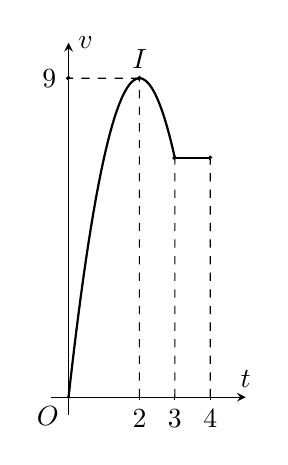
\begin{tikzpicture}[>=stealth,scale=0.45]
% Vẽ 2 trục, điền các số lên trục
\draw[->] (-0.5,0)--(0,0) node[below left]{$O$}--(5,0) node[above]{$t$};
\foreach \x in {2,3,4}
\draw[shift={(\x,0)},color=black] (0pt,2pt)--(0pt,-2pt)
node[below] { $\x$};
\draw[->,color=black] (0,-0.5)--(0,10) node[right]{$v$};
\foreach \y in {9}
\draw[shift={(0,\y)},color=black] (2pt,0pt) -- (-2pt,0pt)
node[left] {$\y$};
\clip(-1,-1) rectangle (5,10); %vùng đồ thị
%\draw[gray!50,thin,opacity=.5] (-1,-1) grid (4,10); %ô vuông
%Vẽ đồ thị
\draw[smooth,samples=100,domain=0:3, font=\footnotesize, line join=round, line cap=round, thick, smooth]
plot(\x,{(-9/4)*(\x)^2+9*(\x)});
\draw[smooth,samples=100, font=\footnotesize, line join=round, line cap=round, thick, smooth,domain=3:4]
plot(\x,{27/4});
% Vẽ thêm mấy cái râu ria
\draw[dashed] (3,0)--(3,27/4) circle(1.5pt);  \draw[dashed] (2,0)--(2,9) circle(1.5pt) node[above]{$I$}--(0,9) circle(1.5pt); \draw[dashed] (4,0)--(4,27/4) circle(1.5pt);
%Vẽ dấu chấm tròn
\fill (0cm,0cm) circle (1.5pt);
\end{tikzpicture}
\end{center}
\shortans{$27$}
\loigiai{
Gọi $\left(P\right) \colon y = ax^2+bx+c$.\\
Vì $\left(P\right)$ qua $O\left(0;0\right)$ và có đỉnh $I\left(2;9\right)$ nên dễ tìm được phương trình là $y = \dfrac{-9}{4}x^2 + 9x$.\\
Ngoài ra tại $x=3$ ta có $y = \dfrac{27}{4}$.\\
Vậy quãng đường cần tìm là: $S = \displaystyle\int\limits_0^3 \left(\dfrac{-9}{4}x^2 +9x \right) \mathrm{\,d}x + \displaystyle\int\limits_3^4 \dfrac{27}{4} \mathrm{\,d}x = 27$ (km).
}
\end{ex}

\begin{ex}%[EX-Ôn Tập TN 2025,  Lê Hoàng Anh]%[2H5V2-8]
    Trong không gian $Oxyz$, đài kiểm soát không lưu sân bay có toạ độ $O(0;0;0)$, đơn vị trên mỗi trục tính theo kilômét. Một máy bay chuyển động hướng về đài kiểm soát không lưu, bay qua hai vị trí $A(-500;-250;150)$, $B(-200;-200;100)$. Khi máy bay ở gần đài kiểm soát nhất, toạ độ của vị trí máy bay là $(a;b;c)$. Biết rằng $a-b+c=\dfrac{m}{n}$, tính giá trị biểu thức $m-n$?
    \shortans{$4\,881$}
    \loigiai{
    Véc-tơ $\overrightarrow{AB}=(300;50;-50)$ nên $\overrightarrow{u}=(6;1;-1)$ là một véc-tơ chỉ phương của đường thẳng $AB$.\\
    Phương trình đường thẳng $AB$ là
    \[
    \dfrac{x+500}{6}=\dfrac{y+250}{1}=\dfrac{z-150}{-1}.
    \]
    Gọi $H$ là hình chiếu của điểm $O$ trên đường thẳng $AB$ thì $OH$ là khoảng cách ngắn nhất giữa máy bay và đài kiểm soát. Khi đó $H(6t-500;t-250;-t+150)$.\\
    Ta có $\overrightarrow{OH} \cdot \overrightarrow{u}=(6t-500) \cdot 6+t-250-(-t+150)=0 \Leftrightarrow t=\dfrac{1\,700}{19}$.\\
    Suy ra toạ độ của vị trí máy bay khi đó là $\left(\dfrac{700}{19};\dfrac{-3\,050}{19};\dfrac{1\,150}{19}\right)$.\\ Vậy $a-b+c= \dfrac{4\,900}{19}$, suy ra $m-n=4\,881$.
    }
    \end{ex}

\begin{ex}%[2D6V1-3]
Tất cả các học sinh của trường Hạnh Phúc đều  tham gia câu lạc bộ bóng chuyền hoặc bóng rổ, mỗi học sinh chỉ tham gia đúng $1$ câu lạc bộ. Có $60$\% học sinh của trường tham gia câu lạc bộ bóng chuyền và $40$\% học sinh của trường tham gia câu lạc bộ bóng rổ. Số học sinh nữ chiếm $65$\% trong câu lạc bộ bóng chuyền và $25$\% trong câu lạc bộ bóng rổ. Chọn ngẫu nhiên $1$ học sinh. Xác suất chọn được học sinh nữ là bao nhiêu?

\shortans{0,49}
\loigiai
{
Gọi $A$ là biến cố \textquotedblleft Số học sinh thuộc câu lạc bộ bóng chuyền\textquotedblright.\\
$B$ là biến cố \textquotedblleft Số học sinh nữ\textquotedblright.\\
Khi đó $\heva{&P(A) = 60\% = 0{,}6 &\Rightarrow& P(\overline{A}) = 1-0{,}6 = 0{,}4\\ &P(B|A) = 65\% = 0{,}65 &\Rightarrow& P(\overline{B}|A) = 1-0{,}65 = 0{,}35\\ &P(B|\overline{A}) = 25\% = 0{,}25 &\Rightarrow& P(\overline{B}|\overline{A}) = 1-0{,}25=0{,}75.}$
\begin{center}
\begin{tikzpicture}[>=stealth]
%Khung 1
\draw (-0,-1) rectangle (2.2,0);
\draw (1.1,-0.5) node{Gốc};
%Mui ten 1,2
\draw [->] (2.2,-0.5)--(3.8,1.6) node[pos=0.5,sloped,above]{$0{,}6$};
\draw [->] (2.2,-0.5)--(3.8,-2.6) node[pos=0.5,sloped,below]{\color{red}$0{,}4$};
%Khung 2.1
\draw (4.5,3.0) node{\textbf{Thuộc câu lạc bộ}};
\draw (3.8,1.1) rectangle (5.1,2.1);
\draw (8.9/2,1.6) node{$A$} ;
%Khung 2.2
\draw (3.8,-2.1) rectangle (5.1,-3.1);
\draw (8.9/2,-2.6) node{$\overline{A}$};
%Mui ten 3,4
\draw [->] (5.1,1.6)--(6.5,2.6) node[pos=0.5,sloped,above]{$0{,}65$};
\draw [->] (5.1,1.6)--(6.5,0.6) node[pos=0.5,sloped,below]{\color{red}$0{,}35$};
%Mui ten 5,6
\draw [->] (5.1,-2.6)--(6.5,-1.6) node[pos=0.5,sloped,above]{$0{,}25$};
\draw [->] (5.1,-2.6)--(6.5,-3.6) node[pos=0.5,sloped,below]{\color{red}$0{,}75$};
%Khung 3.1
\draw (6.5,2.2) rectangle (7.7,3.2);
\draw (7.1,5.4/2) node{$B$} ;
%Khung 3.2
\draw (7.0,3.7) node{\textbf{Nữ}};
\draw (6.5,1.2) rectangle (7.7,0.2);
\draw (7.1,1.4/2) node{$\overline{B}$} ;
%Khung 3.3
\draw (6.5,-1.1) rectangle (7.7,-2.1);
\draw (7.1,-3.2/2) node{$B$} ;
%Khung 3.3
\draw (6.5,-2.9) rectangle (7.7,-3.9);
\draw (7.1,-3.4) node{$\overline{B}$} ;
%Kết quả
\draw (9.5,3.7) node{\textbf{Kết quả}};
\draw (9.5,2.7) node{$AB$};
\draw (9.5,0.7) node{$A \overline{B}$};
\draw (9.5,-1.6) node{$\overline{A}B$};
\draw (9.5,-3.4) node{$\overline{A}~\overline{B}$};
%Xác suất
\draw (12.5,3.7) node{\textbf{Xác suất}};
\draw (12.5,2.7) node{$0{,}39$};
\draw (12.5,0.7) node{$0{,}21$};
\draw (12.5,-1.6) node{$0{,}1$};
\draw (12.5,-3.4) node{$0{,}3$};
\end{tikzpicture}
\end{center}
Áp dụng công thức xác suất toàn phần để tính xác chọn được học sinh là nữ
\[P(B) = P(A) \cdot P(B|A) + P(\overline{A}) \cdot P(B|\overline{A}) = 0{,}6 \cdot 0{,}65 + 0{,}4 \cdot 0{,}25 = 0{,}49.\]
}
\end{ex}
\TL
\begin{ex}%[2H5H2-3]%[Dự án EX-TF-TLN lần 3 - Nguyen Chín Em]
Trong không gian với hệ tọa độ $Oxyz$. Viết phương trình tham số của $d$ biết $d$ đi qua điểm $M(3; 1; 5)$ và song song với hai mặt phẳng $(P)\colon 2x+3y-2z+1=0$ và $(Q)\colon x-3y+z-2=0$. %Khi đó đường thẳng $d$ đi qua $(6;y_0;z_0)$. Tính $z_0-y_0$.
% \shortans{$9$}
\loigiai{
Ta có  $\overrightarrow{n_P} = (2; 3; -2)$, $\overrightarrow{n_Q} = (1; -3; 1)$ lần lượt là véc-tơ pháp tuyến của hai mặt phẳng $(P)$ và $(Q)$. Do $d \parallel (P)$ và $d \parallel (Q)$ nên véc-tơ chỉ phương của $d$ là $\overrightarrow{u}=\left[\overrightarrow{n_P}, \overrightarrow{n_Q}\right]= (-3; -4; -9)$.\\
Phương trình tham số của $d$ là $\heva{&x = 3 - 3t\\&y = 1 - 4t\\&z = 5 - 9t}, (t\in\mathbb{R})$.\\
Với $t=-1$, suy ra đường thẳng $d$ đi qua $(6;5;14)$. Suy ra được $y_0=5;z_0=14\Rightarrow z_0-y_0=9$.
}
\end{ex}

\begin{ex}%[2D6C2-4]
Ở một khu rừng nọ có $7$ chú lùn, trong đó có $4$ chú luôn nói thật, $3$ chú còn lại nói thật với  xác suất $0{,}5$. Bạn Tuyết gặp ngẫu nhiên một chú lùn. Gọi $A$ là biến cố \lq\lq Chú lùn đó luôn nói thật\rq\rq\,và $B$ là biến cố \lq\lq Chú lùn đó tự nhận mình luôn nói thật\rq\rq. Biết rằng chú lùn mà bạn Tuyết gặp tự nhận mình là người luôn nói thật. Tính xác suất để chú lùn đó luôn nói thật (làm tròn hai chữ số thập phân).
% \shortans{$0{,}73$}
\loigiai{
Ta có $\mathrm{P}(A)=\dfrac{4}{7}$; $\mathrm{P}(\overline{A})=\dfrac{3}{7}$; $\mathrm{P}(B \mid A)=1$; $\mathrm{P}(B \mid \overline{A})=0{,}5$.\\
Theo công thức xác suất toàn phần, ta có
\begin{eqnarray*}
\mathrm{P}(B) & =& \mathrm{P}(A) \cdot \mathrm{P}(B \mid A)+\mathrm{P}(\overline{A}) \cdot \mathrm{P}(B \mid \overline{A}) \\
& = & \dfrac{4}{7} \cdot 1+\dfrac{3}{7} \cdot 0{,}5=\dfrac{11}{14}.
\end{eqnarray*}
Khi đó
\[
\mathrm{P}(A \mid B)=\dfrac{\mathrm{P}(AB)}{\mathrm{P}(B)}=\dfrac{\mathrm{P}(A) \cdot \mathrm{P}(B \mid A)}{\mathrm{P}(B)}=\dfrac{\dfrac{4}{7} \cdot 1}{\dfrac{11}{14}}=\dfrac{8}{11} \approx 0{,}73.
\]
}
\end{ex}

\begin{ex}%[2H5C1-7]
Người ta thiết kế một mái che hình chữ nhật $ ABCD $ phía trên sân khấu. Gắn hệ trục tọa độ $ Oxyz $ (đơn vị trên trục là mét), người ta xác định được toạ dộ của các điểm như sau: $ A(0;0;8)$, $B(0;20;8)$, $D(15;0;14)$, $C(15;20;14) $. Một cổng chào hình chữ nhật $ EFHG $ với tọa độ điểm $ G(8;0;4) $ dựng vuông góc với mặt đất. Người ta muốn làm các đoạn dây nối thanh ngang $ GE $ với mái che để gắn hoa và đèn led. Độ dài ngắn nhất của mỗi đoạn dây này bằng bao nhiêu mét? (làm tròn đến chữ số thập phân thứ nhất)
\begin{center}
\includegraphics[scale=.7]{images/2P5-1-H5-16}
\end{center}
% \shortans{$1{,}8$}
\loigiai{
Ta có $ A(0;0;8)$, $B(0;20;8)$, $D(15;0;14)$, $C(15;20;14) $.\\
Ta có $ \vec{AB}=(0;20;0) $, $\vec{AC}=(15;20;6)$ nên $ \vec{n}_1=\left[\vec{AB},\vec{AC}\right]=(80;0;300) $ là vectơ pháp tuyến của $ (ABCD) $.\\
Mà mặt phẳng mái che $ (ABCD) $ qua $ A(0;0;8)$ nên có phương trình
\[ 80(x-0)+0(y-0)+300(z-8)=0\Leftrightarrow 4x+15z-120=0 .\]
Độ dài ngắn nhất của dây nối thanh ngang $ GE $ với mái che là khoảng cách từ $ G $ đến mái che (mặt phẳng $ ABCD $) là \[ \mathrm{d}(G,(ABCD))=\dfrac{|4\cdot8+0+15\cdot4-120|}{\sqrt{4^2+0^2+15^2}}=\dfrac{28}{\sqrt{241}}=1{,}8\ (\text{m}). \]
}
\end{ex}
\Closesolutionfile{ans}
\Closesolutionfile{ansbook}
